\documentclass[english,a4paper,oneside]{scrbook}
\pagestyle{plain}

\usepackage[citestyle=numeric-comp,style=numeric,giveninits=true,backend=biber,isbn=false,doi=false,dateabbrev=false,url=false]{biblatex}
\usepackage[hidelinks]{hyperref}
\usepackage[nodayofweek]{datetime}
\usepackage{siunitx,color,amsmath,acro,caption,upquote,pdfpages,amsthm,cleveref,amsfonts,stmaryrd,comment}
%\usepackage{listings}
%\usepackage{float}

\newtheorem{theorem}{Theorem}[section]
\newtheorem{remark}[theorem]{Remark}
\newtheorem{notation}[theorem]{Notation}
\newtheorem{lemma}[theorem]{Lemma}
\newtheorem{definition}[theorem]{Definition}
\newtheorem{example}{Example}[theorem]
\newcommand{\f}[1]{#1:\mathbb{R}\rightarrow\mathbb{R}}
\newcommand{\id}{\mathrm{id}_\mathbb{R}}
\newcommand{\Mathref}[1]{\mathrm{\Cref{#1}}}
\newcommand{\E}{\mathrm{E}}
\renewcommand{\d}{\mathrm{d}}
\newcommand{\independent}{\perp\!\!\!\perp}


\hypersetup{
    linktoc=all
}

\addbibresource{paper.bib}

\hyphenation{}

\author{Nicholas-Philip Brandt}
\title{Bell's inequality and its violation}

%\chapter*{Acronyms}
%\addcontentsline{toc}{chapter}{Acronyms}

\DeclareAcronym{DAG}{
short = DAG,
long = directed acyclic graph
}

\DeclareAcronym{CI}{
short = CI,
long = conditional independence
}

\DeclareAcronym{EPR}{
short = EPR,
long = Einstein-Podolsky-Rosen
}

\DeclareAcronym{CHSH}{
short = CHSH,
long = Clauser-Horne-Shimony-Holt
}

\DeclareAcronym{CDA}{
short = CDA,
long = causal discovery algorithm
}

%\begin{acronym}[acronyms]
%\acro{DAG}{directed acyclic graph}
%\acro{CI}{conditional independence}
% \acroplural{CI}{conditional independences}
%\acro{EPR}{Einstein-Podolsky-Rosen}
%\acro{CHSH}{Clauser-Horne-Shimony-Holt}
%\acro{CDA}{causal discovery algorithm}
%\end{acronym}

\begin{document}

\maketitle

\frontmatter
\setcounter{page}{1}
\pagenumbering{roman}
\tableofcontents

\mainmatter
\chapter{Basics}
\label{Basics}

\section{Causal Structure and Models}
\label{Basics:CausalModels}

A causal structure is a set of random variables $V$ and pairs of those variables $E\subset V^2$ which correspond to direct causations between them.
Naturally, a causal structure is a \ac{DAG}.
A causal model $M=(G,\Theta)$, however, consists of a causal structure $G=(V,E)$ and causal-statistical parameters $\Theta$.
Causal-statistical parameters specify the conditioned probabilities $P(X|\mathrm{Pa}(X))$ of any variable $X$ given its parent variables $\mathrm{Pa}(X)$ (direct causes).
In other words: The causal structure dictates \textbf{if} a variable causally influences another variable while the causal-statistical parameters dictate \textbf{how} the influence looks like. \cite{Wood.2015}

\section{Local Hidden-Variable Theories}
\label{Basics:LocalHiddenVariableTheories}

Local hidden-variable theories are physical theories that emerged during the first half of the 20th century in an attempt to explain the observed probabilistic nature of certain experiments (e.g. the Stern-Gerlach experiment) in a completely deterministic manner.
This class of theories has physical properties which represent the manifestation of its underlying causal structure.
Subsequently, these three properties, cumulatively called \textbf{local realism}, are listed and described in the following.
classical theories like electromagnetism by Maxwell's equations obey local realism.

\subsection{Locality}
\label{Basics:Locality}

Locality is a property of physical theories that states that nothing, especially no information signal, can propagate through space faster than the speed of light in vacuum.
This means that an event \textbf{cannot} have an immediate (instantaneous) effect on a however distant system.

\subsection{Realism}
\label{Basics:Realism}

Realism is a property of physical theories that states that the result of an interaction of a system is predetermined independently of the actual interaction. This means that the result of any measurement is fixed before the measurement is even performed.
Newtonian mechanic, for example, is a realistic theory in which the mass and velocity predetermine the path of a system through space-time.

\subsection{Freedom of Choice}
\label{Basics:FreedomofChoice}

Freedom of choice in this context refers to the ability to attain (real) random values.
This assumption requires the existence of randomness and rules out so-called superdeterminism which means that the evolution of the entire universe is completely predetermined and predictable if one had knowledge over the state of the entire universe at one moment in time (Laplace's demon).

\begin{comment}
\section{Photons and Filters}
\label{Basics:PhotonsandFilters}

Photons are discrete quanta of the electromagnetic field. For this work it's sufficient to regard photons as particles with a direction of propagation and a polarization in the perpendicular plane.
Polarization filters are devices that have a fixed direction of polarization. Photons that interact with the filter with absolutely the same polarization then the photon is ideally transmitted. A photon with perpendicular polarization will certainly be absorbed by the filter. For photons with an other polarization there's a certain chance of passing through. An ideal filter does not reflect any photons.
\end{comment}

\chapter{Bell's Theorem}
\label{BellsTheorem}

John Stewart Bell formalized 1964 \cite{Bell.1964} Bell's theorem which proofs that no local hidden-variable theory can properly describe the behavior of quantum mechanic systems.
He derived the inequality from the temporal-spatial assumptions of the local hidden-variable theory and showed its violation in certain experiments theoretically.
In 2015 Hensen et al. \cite{Hensen.2015} demonstrated a loophole-free violation of Bell's inequality.

\section{Causal Struture and Inequality}
\label{Basics:CausalStructure}

\begin{figure}[t!]
\centering
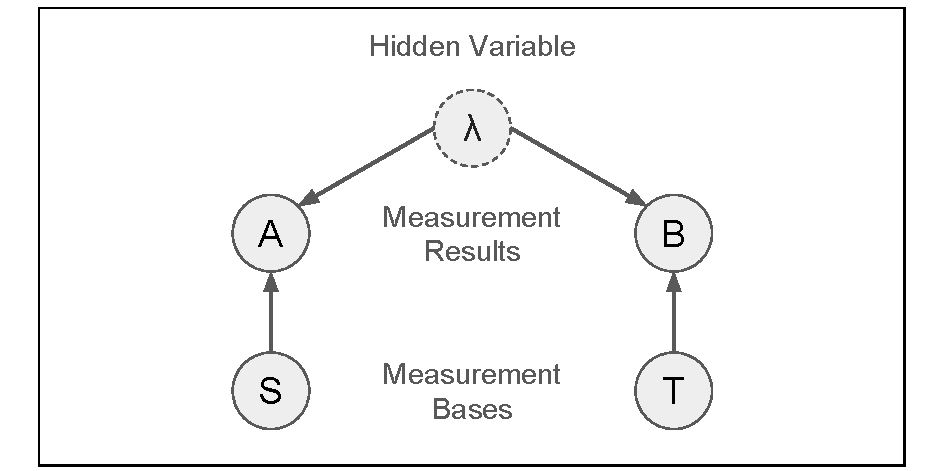
\includegraphics[width=\textwidth,height=200px,keepaspectratio]{images/CSofLHVT}
\caption{Causal structure of local hidden-variable theories}
\label{fig:CSofLHVT}
\end{figure}

The causal structure of local hidden-variable theories is shown in \ref{fig:CSofLHVT}.
Applying the causal Markov condition to this causal structure leads to the following \acp{CI}:

\begin{equation}
\begin{aligned}
A\independent&\ BT\ |\ \lambda S
\\
B\independent&\ AS\ |\ \lambda T
\\
\lambda\independent&\ ST
\\
S\independent&\ \lambda BT
\\
T\independent&\ \lambda AS
\end{aligned}
\end{equation}
These \acp{CI} are purely mathematical consequences.
The temporal-spatial assumptions which Bell appealed to are merely manifestations of those underlying \acp{CI}.
For example the realism property is reflected in $\lambda\independent\ ST$ which states that the hidden variable of a system is not influenced by the choice of measurement prior to the measurement itself.
Another property, namely freedom of choice, is build in the model itself in the way that the choice of measurement bases is even presentable as random variables.

However, a superset of inequalities (containing the historic Bell inequality) can be derived solely from the causal structure of local hidden-variable theories.
In the following a form of Bell's inequality for the expectation values of correlations is deduced using an algebraic inequality.

\begin{lemma}
\label{lemma:UVW}
UVW Inequality

Let $U,V,W\in[-1,1]$ be three arbitrary real numbers, then the algebraic equation
\begin{equation}
U\cdot V-U\cdot W+V\cdot W
\leq1
\end{equation}
holds.

\begin{proof}
Firstly, the inequality
\begin{equation}
U\cdot V-U\cdot W+V\cdot W
=V\cdot(U+W)-U\cdot W
\leq |U+W|-U\cdot W
\end{equation}
is split in to cases.
In both the first case
\begin{multline}
U+W
\geq0
\\
\Rightarrow
U\cdot V-U\cdot W+V\cdot W
\leq U+W-U\cdot W
=\underbrace{(U-1)\cdot(1-W)}_{\leq0}+1
\leq1
\end{multline}
and in the second case
\begin{multline}
U+W
\leq0
\\
\Rightarrow
U\cdot V-U\cdot W+V\cdot W
\leq -U-W-U\cdot W
=\underbrace{-(1+U)\cdot(1+W)}_{\leq0}+1
\leq1
\end{multline}
the inequality holds.
\end{proof}
\end{lemma}

The image of the random variables $A$ and $B$ is now considered to be limited to $[-1,1]$ because every random variable over the real numbers $\mathbb{R}$ can be transformed into this interval without a loss of cardinality.
Henceforth, the variables $A$ and $B$ may be interpreted as deterministic functions $a:\lambda',s\mapsto a(\lambda',s)$ and $b:\lambda',t\mapsto b(\lambda',t)$ that return their respective result given instantiated values of $\lambda'\leftarrow\lambda$ and $s\leftarrow S$ or $t\leftarrow T$.
Furthermore $\Delta$ denotes the image of $\lambda$ with the arbitrary normalized  probability density function $\int\limits_\Delta f_\lambda(\lambda')\d\lambda'
=1$.
Identifying
\begin{alignat*}{2}
U=a(\lambda',\alpha)=b(\lambda',\alpha)
\\
V=a(\lambda',\beta)=b(\lambda',\beta)
\\
W=a(\lambda',\gamma)=b(\lambda',\gamma)
\end{alignat*}
% Why are a and b equal?
with $\alpha,\beta,\gamma\leftarrow S,T$ \cref{lemma:UVW} gives the inequality
% Must S and T have the same image?
\begin{multline}
a(\lambda',\alpha)\cdot b(\lambda',\beta)-a(\lambda',\alpha)\cdot b(\lambda',\gamma)+a(\lambda',\beta)\cdot b(\lambda',\gamma)
\leq1
\\
\Rightarrow
\int\limits_\Delta\left[a(\lambda',\alpha)\cdot b(\lambda',\beta)-a(\lambda',\alpha)\cdot b(\lambda',\gamma)+a(\lambda',\beta)\cdot b(\lambda',\gamma)\right]f_\lambda(\lambda')\d\lambda'
\\
\leq\int\limits_\Delta f_\lambda(\lambda')\d\lambda'
=1
\ .
\end{multline}
This inequality in turn can be expressed in terms of expectation values of correlations between $A$ and $B$ as
\begin{multline}
\label{eq:BellsInequality}
\int\limits_\Delta\left[a(\lambda',\alpha)\cdot b(\lambda',\beta)-a(\lambda',\alpha)\cdot b(\lambda',\gamma)+a(\lambda',\beta)\cdot b(\lambda',\gamma)\right]f_\lambda(\lambda')\d\lambda'
\\
=
\left\{
\begin{aligned}
\int\limits_\Delta\left[a(\lambda',\alpha)\cdot b(\lambda',\beta)\right]f_\lambda(\lambda')\d\lambda'
\\
-\int\limits_\Delta\left[a(\lambda',\alpha)\cdot b(\lambda',\gamma)\right]f_\lambda(\lambda')\d\lambda'
\\
+\int\limits_\Delta\left[a(\lambda',\beta)\cdot b(\lambda',\gamma)\right]f_\lambda(\lambda')\d\lambda'
\end{aligned}
\right\}
\\
=
%\left\{
%\begin{aligned}
\E_\lambda(A\cdot B|S=\alpha,T=\beta)
%\\
-\E_\lambda(A\cdot B|S=\alpha,T=\gamma)
%\\
+\E_\lambda(A\cdot B|S=\beta,T=\gamma)
%\end{aligned}
%\right\}
\leq1
\ .
\end{multline}
Necessary assumptions for the derivation of this Bell inequality are first of all the causal structure which makes $A$ and $B$ expressible through deterministic functions.
However, this inequality is only one of many producible by this procedure.
Another famous inequality is the \ac{CHSH} inequality which utilizes four algebraic number (measurement bases) \cite{Clauser.1969,Peters.2017}.

\section{Inequality Violation}
\label{Basics:InequalityViolation}

The fact that certain experiments yield correlations that violate Bell's inequality imply that local hidden-variable theories are not able to reproduce the results of those experiments.
This means that the causal structure does not accurately describe the underlying mechanisms of the experiment.

Bell originally demonstrated \cite{Bell.1964} the violation for the so-called \ac{EPR} experiment.
For this experiment the correlation of the two measurement result has experimentally found to be \begin{equation}
\label{eq:EPRCorrelation}
\E(A\cdot B|S=\alpha,T=\beta)=\cos\theta_{\vec\alpha\vec\beta}
\end{equation}
for given polarization values $\alpha$ and $\beta$ where $\theta_{\vec\alpha\vec\beta}$ denotes the angle between them.
Simply inserting this value in the inequality gives
\begin{multline}
\E_\lambda(A\cdot B|S=\alpha,T=\beta)
-\E_\lambda(A\cdot B|S=\alpha,T=\gamma)
+\E_\lambda(A\cdot B|S=\beta,T=\gamma)
\\
=\cos\theta_{\vec\alpha\vec\beta}
-\cos\theta_{\vec\alpha\vec\gamma}
+\cos\theta_{\vec\beta\vec\gamma}
\leq1
\ .
\end{multline}
If the theory described the results of the experiment correctly, then the inequality would hold for all angles $\alpha$, $\beta$ and $\gamma$.
However, by choosing $2\theta_{\vec\alpha\vec\beta}=\theta_{\vec\alpha\vec\gamma}=2\theta_{\vec\beta\vec\gamma}=\frac{\pi}{3}$ the inequality is finally violated
\begin{equation}
\underbrace{\cos\theta_{\vec\alpha\vec\beta}}_{\frac{1}{2}}
-\underbrace{\cos\theta_{\vec\alpha\vec\gamma}}_{-\frac{1}{2}}
+\underbrace{\cos\theta_{\vec\beta\vec\gamma}}_{\frac{1}{2}}
\leq1
\ \lightning
\ .
\end{equation}

\chapter{Causal Discovery Algorithms}
\label{CausalDiscoveryAlgorithms}

Normally, scientists and engineers try to infer information about the behavior of a system using (partial) knowledge about the causal structure.
An example of this workflow is the analysis of a CMOS AND gate.
Using the knowledge about the electrical components (transistors, diodes, etc.) it's possible to estimate the output statistics for given inputs.

Causal discovery algorithms, however, seek to solve the inverse problem.
They are heuristic tools to extract the causal structure from given correlations.

It's interesting to see which conclusions a \acl{CDA} might draw from correlations that violate Bell inequalities.
\Aclp{CDA} might prove useful in the pursuit of understanding the causal structure of quantum governed systems.
Because of Bell's theorem their behavior is not explicable by the causal structure of local hidden-variable theories.

\section{Faithfulness}
\label{Basics:Faithfulness}

Standard causal discovery algorithms assume faithful probability distribution.

\begin{figure}[b!]
\centering
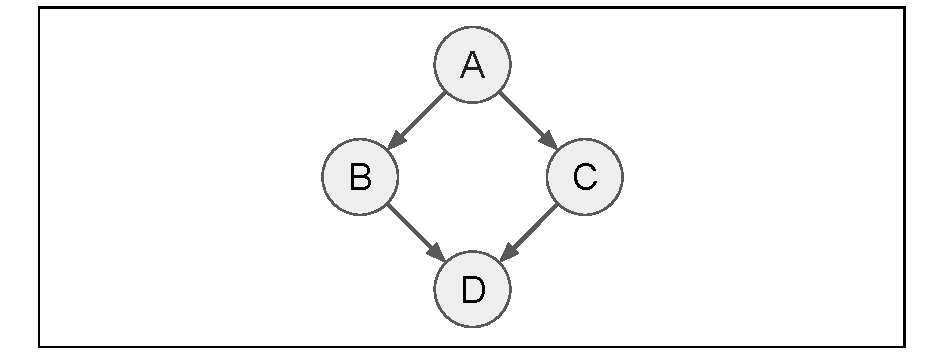
\includegraphics[width=\textwidth,height=180px,keepaspectratio]{images/Unfaithful}
\caption{Causal structure to demonstrate unfaithful distributions}
\label{fig:Unfaithful}
\end{figure}

\begin{definition}
\label{Faithfulness}
Faithfulness (derived from Wood and Spekkens \cite{Wood.2015})

The probability distribution induced by a causal model $M$ (over the
variables in M or some subset thereof) is faithful if its CIs continue to hold for
any variation of the causal-statistical parameters $\Theta$ in $M$.
\end{definition}

This means that the \acp{CI} are truly results of the causal structure and not coincident artifacts of a specific probability distribution.
An example of a unfaithful distribution would be the causal structure \ref{fig:Unfaithful} with the following causal-statistical parameters
\begin{equation}
\Theta
=
\left\{
\begin{aligned}
B&=A,
\\
C&=-A,
\\
D&=B+A=0
\end{aligned}
\right\}
\ .
\end{equation}
Even though the structure suggests a causal influence of $A$ on $D$ these specific causal-statistical parameters lead to $A\independent D$ because $D=0$ in every case.
For the causal-statistical parameters
\begin{equation}
\Theta
=
\left\{
\begin{aligned}
B&=A,
\\
C&=A,
\\
D&=B+A=2A
\end{aligned}
\right\}
\end{equation}
$D$ is obviously depends on $A$.

In order not to be tricked by an unfaithful distribution standard \aclp{CDA} must only regard the \acp{CI} that hold for all causal-statistical parameters (\cref{Faithfulness}).
This limitation will prove to be a critical deficiency in the pursuit of discovering quantum causal structures. 
An implemented algorithm given a finite set of data cannot vary the statistical-parameters and is therefore forced to assume faithfulness of the given correlations.
Unfortunately, for any unfaithful input these algorithms do not recognize its unfaithfulness but rather output (possibly a set of) causal structures that seem valid but might not reflect the correct causations that generated the input.

\section{Application to Bell-Violating Correlations}
\label{Basics:ApplicationtoBell-ViolatingCorrelations}

\begin{figure}[b!]
\centering
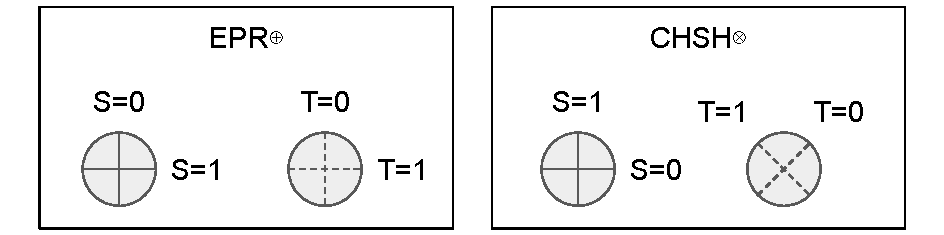
\includegraphics[width=\textwidth]{images/EPRvsCHSH}
\caption{Measurement bases of the EPR (left) and CHSH (right) experiment}
\label{fig:EPRvsCHSH}
\end{figure}

In order to gain understanding about the causal structure of quantum systems an experiment manifesting quantum correlations must be subjected to \acp{CDA} and its output must be interpreted physically.
Another approach following \cite{Wood.2015} is to look at the difference of output for classical correlations (where Bell's inequality holds) and quantum correlations (where Bell's inequality is violated).

Therefore two variants of the \ac{EPR} experiment are considered: Firstly the \ac{EPR}$\oplus$ experiment \cite{Einstein.1935} and secondly the CHSH$\otimes$ experiment \cite{Clauser.1969} both with limitations to the set of their measurement bases.
The setup of these experiments follow the structure \ref{fig:CSofLHVT}; there exist two measurement result $A$ and $B$ and their respective measurement bases $S$ and $T$.
Here $S$ and $T$ only map to $\{0,1\}$ corresponding to two different polarizations of detectors.
A graphical representation of the respective measurement bases is given in figure \ref{fig:EPRvsCHSH}.
In the \ac{EPR}$\oplus$ experiment both detectors can be oriented vertically or horizontally depending on $S$ and $T$.
The \ac{CHSH}$\otimes$ experiment is a derivation of this experiment but the right detector can only be oriented diagonally (meaning $\frac{\pi}{4}\ \widehat{=}\ \ang{45}$ for $T=0$ or $\frac{3\pi}{4}\ \widehat{=}\ \ang{135}$ for $T=1$).
The exact setup and process of these experiment is irrelevant to this work and may be researched in the respective literature.

Of great importance are solely the correlations between the measurement results $A$ and $B$ given their measurement bases $S$ and $T$.
They are experimentally determined by equation \eqref{eq:EPRCorrelation}.
In case of  the \ac{EPR}$\oplus$ experiment correlations are
\begin{equation}
\begin{alignedat}{4}
\E(A\cdot B|S=T)&=\cos0&=1&
\\
\E(A\cdot B|S\neq T)&=\cos\frac{\pi}{2}&=0&
\end{alignedat}
\end{equation}
while the \ac{CHSH}$\otimes$ correlations are 
\begin{equation}
\begin{alignedat}{3}
\E(A\cdot B|S=0,T=0)&=\cos\frac{\pi}{4}&=\frac{1}{\sqrt2}&
\\
\E(A\cdot B|S=0,T=1)&=\cos\frac{\pi}{4}&=\frac{1}{\sqrt2}&
\\
\E(A\cdot B|S=1,T=0)&=\cos\frac{\pi}{4}&=\frac{1}{\sqrt2}&
\\
\E(A\cdot B|S=1,T=1)&=\cos\frac{3\pi}{4}&=-\frac{1}{\sqrt2}&
\  .
\end{alignedat}
\end{equation}
Recall equation \eqref{eq:BellsInequality}; for \ac{EPR}$\oplus$ all possible cases
\begin{equation}
\begin{alignedat}{4}
&\alpha=\beta=\gamma
\Rightarrow&
1-1+-1=1&\leq1
\\
&\alpha=\beta\neq\gamma
\Rightarrow&
1-(-1)-1=1&\leq1
\\
&\alpha\neq\beta=\gamma
\Rightarrow&
-1-(-1)+(-1)=1&\leq1
\\
&\alpha\neq\beta\neq\gamma
\Rightarrow&
-1-1-1=-3&\leq1
\end{alignedat}
\end{equation}
the inequality also holds. So the \ac{EPR}$\oplus$ experiment respects Bell's inequality meaning it's explicable by classical theories.
Consider $\alpha=\gamma=1$ and $\beta=0$ for \ac{CHSH}$\otimes$; for these measurement bases the Bell inequality \eqref{eq:BellsInequality} becomes
\begin{equation}
\frac{1}{\sqrt2}-\left(-\frac{1}{\sqrt2}\right)+\frac{1}{\sqrt2}
=\frac{3}{\sqrt2}
\leq1
\ \lightning
\end{equation}
which obviously violates the inequality. Thus classical theories cannot explain the \ac{CHSH}$\otimes$ experiment.
However, both experiments yield exactly the \textbf{same} \acp{CI}
\begin{equation}
\label{eq:CIs}
(S\independent T),
(A\independent T\ |\ S),
(B\independent S\ |\ T)
\ .
\end{equation}
These are not all \acp{CI} but rather a generating set from which all can be inferred by the semi-graphoid axioms \cite{Wood.2015}.
Although one experiment is explicable by classical theories and one is not faithful \aclp{CDA} will draw the \textbf{same} conclusions from them.
This in turn means that faithful \aclp{CDA} cannot produce any new information about the quantum causal structure that it did not produce for classical correlations beforehand.

Finally, Wood and Spekkens \cite{Wood.2015} conclude from these theoretical results that \acp{CI} alone do not provide enough information about the quantum causal structure.
Therefore a \ac{CDA} that may explain that structure must include the strength of the correlations as well as the \acp{CI}, reintroducing the problem of faithfulness.

\chapter{Summary}
\label{Summary}

Historically, Bell's inequality is one of the most crucial tools in the pursuit to understand quantum theory because it categorically rules out the whole class of local hidden-variable theories.
However, in the context of the comparatively young field of causal inference Bell's inequality is only one of many inequalities that arise purely from a causal structure and algebraic inequalities.
Due to this fact Bell's and similar inequalities can be used to test the ability of many causal structures to generate quantum correlations in various setups.

In conclusion, any \ac{CI}-based \ac{CDA} cannot distinguish quantum (Bell-violating) correlations from classical (Bell-satisfying) correlations due to insufficient information provided by \acp{CI} from the Markov condition. Solely based on the information provided by the \acp{CI} \eqref{eq:CIs} the faithful algorithms will draw the same conclusions about the underlying causal structure, meaning both correlations inherit the same causal structure.\\
More importantly, the hidden-variable causal structure (figure \ref{fig:CSofLHVT}) cannot generate quantum correlations because they violate Bell's inequality.
To be able to generate quantum correlations additional edges in the \ac{DAG} of the quantum causal structure (e.g. superluminal signaling from $S$ to $B$) are necessary; thus violating the faithfulness of observed \acp{CI} relative to the extended \ac{DAG}.
To gain understanding about the quantum causal structure it is necessary to take the strength of correlations into account which contradicts the sole dependency of the \acp{CDA} on \acp{CI} \cite{Wood.2015}.
A new approach heeding the strength of correlations but immune to unfaithful correlations is needed to solve this dilemma.

\printbibliography[heading=bibintoc]

\listoffigures

\newpage
\addcontentsline{toc}{chapter}{Acronyms}
\printacronyms

% \listoftables
% \chapter*{Formelverzeichnis}
\addcontentsline{toc}{chapter}{Formelverzeichnis}

\newcommand{\acrounit}[1]{
  \acroextra{\makebox[18mm][l]{\si{#1}}}
}

\begin{acronym}[acronyms]

\acro{A_Det}[\ensuremath{A_\mathrm{Det}}]{\acrounit{m^2} Detektorfläche}
\acro{C_12}[\ensuremath{C_{12}}]{\acrounit{} Transmission des Zirkulator von Eingang 1 zu 2}
\acro{C_23}[\ensuremath{C_{23}}]{\acrounit{} Transmission des Zirkulator von Eingang 2 zu 3}
\acro{CR}[\ensuremath{CR}]{\acrounit{Hz} Zählrate}
\acro{DCR}[\ensuremath{DCR}]{\acrounit{Hz} Dunkelzählrate}
\acro{DE}[\ensuremath{DE}]{\acrounit{} Detektionseffizienz}
\acro{E_Ph}[\ensuremath{E_\mathrm{Ph}}]{\acrounit{} Photonenenergie}
\acro{G(r)}[\ensuremath{G(r)}]{\acrounit{\frac{W}{m^2}} Näherung der Intensität unter dem Objektiv}
\acro{h}[\ensuremath{h}]{\acrounit{\mathbb{Z}} Zeilenanzahl bei Rasterverfahren}
\acro{I(r)}[\ensuremath{I(r)}]{\acrounit{\frac{W}{m^2}} Intensität unter dem Objektiv}
\acro{I_0}[\ensuremath{I_0}]{\acrounit{\frac{W}{m^2}} Maximalintensität}
\acro{I_B}[\ensuremath{I_\mathrm{B}}]{\acrounit{A} Biasstrom}
\acro{I_C}[\ensuremath{I_\mathrm{C}}]{\acrounit{A} kritischer Biasstrom}
\acro{IDE}[\ensuremath{IDE}]{\acrounit{} Intrisische Detektionseffizienz}
\acro{j_min}[\ensuremath{j_\mathrm{min}}]{\acrounit{\mathbb{Z}} Schutzschrittzahl}
\acro{f_Laser}[\ensuremath{f_\mathrm{Laser}}]{\acrounit{Hz} Repetitionsrate des Lasers}
\acro{f_Piezo}[\ensuremath{f_\mathrm{Piezo}}]{\acrounit{Hz} Sägezahnfrequenz der Piezomotoren}
\acro{l}[\ensuremath{l}]{\acrounit{m} Detektorlänge in Y-Richtung}
\acro{L}[\ensuremath{L(\vec{s})}]{\acrounit{m} Länge eines Ansteuerungsschritts}
\acro{N_Pulse}[\ensuremath{N_\mathrm{Pulsel}}]{\acrounit{\mathbb{Z}} Anzahl der Pulse in einer \ac{CR}-Samplemessung}
\acro{N_Samples}[\ensuremath{N_\mathrm{Samples}}]{\acrounit{\mathbb{Z}} Anzahl der \ac{CR}-Samplemessungen}
\acro{NA}[\ensuremath{NA}]{\acrounit{} Numerische Aperatur der Fokuslinse}
\acro{p_y}[\ensuremath{p_\mathrm{y}}]{\acrounit{} Position in Y-Richtung}
\acro{P_Det}[\ensuremath{P_\mathrm{Det}}]{\acrounit{W} Leistung auf dem Detektor}
\acro{P_Untergrund}[\ensuremath{P_\mathrm{Untergrund}}]{\acrounit{W} Leistung auf dem Untergrund}
\acro{PCR}[\ensuremath{PCR}]{\acrounit{Hz} Photonenzählrate}
\acro{r_0}[\ensuremath{r_0}]{\acrounit{m} Radius der ersten Airydisk}
\acro{s}[\ensuremath{\vec{s}}]{\acrounit{\mathbb{Z}^3} Steuerungsvektor}
\acro{SDE}[\ensuremath{SDE}]{\acrounit{} Systemdetektionseffizienz}
\acro{SSD_k(nu)}[\ensuremath{SSD_\mathrm{k}(\nu)}]{\acrounit{W^2} \acl{SSD}: Ähnlichkeitsmaß}
\acro{T_Diode}[\ensuremath{T_\mathrm{Diode}}]{\acrounit{} Transmission vom Untergrund zur Photodiode}
\acro{T_Obj}[\ensuremath{T_\mathrm{Obj}}]{\acrounit{} Transmission des Objektivs}
\acro{T_Stab}[\ensuremath{T_\mathrm{Stab}}]{\acrounit{} Transmission der Stabfaser}
\acro{T_Untergrund}[\ensuremath{T_\mathrm{Untergrund}}]{\acrounit{} Transmission des Systemeingangs bis zum Untergrund}
\acro{U_Piezo}[\ensuremath{U_\mathrm{Piezo}}]{\acrounit{V} Spannungsamplitude (Stepping-Modus) der Piezomotoren}
\acro{U_Schwell}[\ensuremath{U_\mathrm{Schwell}}]{\acrounit{V} Schwellspannung des Pulscounters}
\acro{U_x}[\ensuremath{U_\mathrm{x}}]{\acrounit{V} Spannungsamplitude der Piezomotor in X-Richtung}
\acro{U_y}[\ensuremath{U_\mathrm{y}}]{\acrounit{V} Spannungsamplitude der Piezomotor in Y-Richtung}
\acro{U_z}[\ensuremath{U_\mathrm{z}}]{\acrounit{V} Spannungsamplitude der Piezomotor in Z-Richtung}
\acro{w}[\ensuremath{w}]{\acrounit{m} Detektorbreite in X-Richtung}
\acro{x}[\ensuremath{x}]{\acrounit{\mathbb{Z}} Stick-Slip-Zyklen pro Ansteuerungskommando in X-Richtung}
\acro{y}[\ensuremath{y}]{\acrounit{\mathbb{Z}} Stick-Slip-Zyklen pro Ansteuerungskommando in Y-Richtung}
\acro{z}[\ensuremath{z}]{\acrounit{\mathbb{Z}} Stick-Slip-Zyklen pro Ansteuerungskommando in Z-Richtung}
\acro{beta}[\ensuremath{\beta}]{\acrounit{} Asymmetriefaktor}
\acro{beta_x(k)}[\ensuremath{\tilde\beta_\mathrm{x}(k)}]{\acrounit{} Asymmetriefaktor in X-Richtung in stabilem Raster}
\acro{delta_k}[\ensuremath{\delta_\mathrm{k}}]{\acrounit{m} Positionsabweichung nach $k$-ter kompletter Messzeile}
\acro{eta_Splitter}[\ensuremath{\eta_\mathrm{Splitter}}]{\acrounit{} Leistungsverhältnis des Beamsplitters}
\acro{phi_qDet}[\ensuremath{\phi_\mathrm{q,Det}}]{\acrounit{Hz} Photonenfluss auf den Detektor}
\acro{phi_qSystem}[\ensuremath{\phi_\mathrm{q,System}}]{\acrounit{Hz} Photonenfluss in das System (Messstab)}
\acro{lambda}[\ensuremath{\lambda}]{\acrounit{m} Wellenlänge der Photonen}
\acro{rho_IDE}[\ensuremath{\rho_\mathrm{IDE}}]{\acrounit{m^{-2}} Lokale, intrisische Detektionseffizienz}
\acro{sigma}[\ensuremath{\sigma}]{\acrounit{m} Standardabweichung der Näherung der Intensität}
\acro{tau_Laser}[\ensuremath{\tau_\mathrm{Laser}}]{\acrounit{s} Pulslänge des Lasers}
\acro{tau_Sprung}[\ensuremath{\tau_\mathrm{Sprung}}]{\acrounit{s} Sprungdauer der Sägezahnspannung der Piezomotoren}
\acro{theta}[\ensuremath{\theta_j}]{\acrounit{} Standardabweichungen des aktuellen Zählers}
\acro{u(k)}[\ensuremath{u(k)}]{\acrounit{m} Position in X-Richtung nach $k$ einfachen Zeilenmessungen}
\acro{zeta_x}[\ensuremath{\zeta_\mathrm{x}}]{\acrounit{} Rundungsfehler in X-Richtung in Einheiten von Schrittlängen}
\acro{U}[\ensuremath{\mathcal{U}}]{\acrounit{} Menge aller konfigurierten Schwellspannungen}
\end{acronym}
% \appendix
% \input{sections/appendix.tex}

\end{document}
